\documentclass[a4paper]{article}

%% Language and font encodings
\usepackage[english]{babel}
\usepackage[utf8]{inputenc}
\usepackage[T1]{fontenc}
\usepackage{amsfonts}

%% Sets page size and margins
\usepackage[a4paper,top=3cm,bottom=2cm,left=3cm,right=3cm,marginparwidth=1.75cm]{geometry}

%% Useful packages
\usepackage{amsmath}
\usepackage{amssymb}
\usepackage{amsthm}
\usepackage{graphicx}
\usepackage[colorinlistoftodos]{todonotes}
\usepackage[colorlinks=true, allcolors=blue]{hyperref}

%% Table packages
\usepackage{array}
\newcolumntype{P}[1]{>{\centering\arraybackslash}p{#1}}
\usepackage{multirow}

\title{Mathematical and Physical Modeling of Entangled Photon Propagation in Optical Fibers for MATLAB Simulation}
\author{Marco Cioci\\
Politecnico di Milano\\
Student ID: 10694772\\
\texttt{marco.cioci@mail.polimi.it}}
\date{}

\begin{document}
\maketitle

\tableofcontents

%========================================================
\newpage
\section{General Framework}

\subsection{Purpose and Scope}
The purpose of this document is to define a coherent working framework for the mathematical modeling and numerical simulation of polarization-entangled photon pairs propagating through optical fibers.

This text is not intended to appear directly in the final thesis manuscript. Instead, it serves as an internal technical guide throughout the development of the project. Its role is to support communication, maintain consistency of notation and assumptions, and provide a stable reference for the progressive validation of both the theoretical model and the MATLAB implementation.

The central objective is to organize the physical assumptions, mathematical formalism, and simulation strategy into a reproducible structure, so that each computational step can be traced back to a precise theoretical element. In this way, the simulator is not developed as an isolated numerical tool, but as a direct operational translation of the underlying quantum model.

\paragraph{Simulation notes.}
At the MATLAB level, this document should be treated as the reference specification for notation, model hierarchy, and implementation priorities. The simulator should therefore be organized into clearly identifiable modules, each corresponding to a specific theoretical block. This modular structure is essential both for step-by-step validation of intermediate results and for future extensions of the model, such as the inclusion of mixed states, decoherence mechanisms, and more realistic fiber-channel descriptions.

\subsection{Theoretical Formalism and Notation}

The system is described within the framework of quantum information theory. The relevant mathematical structures include finite-dimensional Hilbert spaces, quantum states, tensor products, unitary operators, density operators, and projective measurements. Elements of classical optics are introduced only when required to justify the physical origin of the effective quantum transformations.

The notation and formal tools are aligned, as far as possible, with the framework of \textit{Quantum Computation and Quantum Information} by Nielsen and Chuang.

In this formalism:
\begin{itemize}
    \item single subsystems are represented by vectors in \(\mathbb{C}^2\),
    \item composite systems are described by tensor-product spaces,
    \item evolutions are represented by linear operators (unitary in the ideal case),
    \item measurements are described through Hermitian operators.
\end{itemize}

All states and operators are represented as vectors and matrices over \(\mathbb{C}\), with dimensions determined by the tensor-product structure of the system.

\paragraph{Simulation notes.}
The simulator adopts a quantum-information-oriented representation from the outset. Pure states are represented as complex vectors, mixed states as density matrices, and evolutions and measurements as matrix operators.

This abstract structure defines the numerical backbone of the simulator and is independent of the specific physical encoding used.


\subsection{Physical Scenario and Experimental Setting}

The physical setting considered in this work is the following. A spontaneous parametric down-conversion (SPDC) source generates pairs of polarization-entangled photons, ideally prepared in a Bell state. The two photons are injected into distinct optical paths, denoted \(A\) and \(B\), and propagate through independent optical fibers.

Each fiber acts on the polarization degree of freedom of the corresponding photon. In a general description, this action can be represented by a unitary operator acting on a single-qubit Hilbert space. However, motivated by experimental constraints and by the limited degree of control available on the full polarization transformation, the model is initially restricted to a simplified effective description.

After compensation of global polarization rotations, the dominant residual effect can be modeled as a relative phase shift between the horizontal and vertical polarization components. In the qubit representation, this corresponds to a rotation around the computational \(Z\)-axis of the Bloch sphere.

The objective at this stage is therefore not to reproduce the full electromagnetic propagation in optical fibers, but to construct an effective quantum model that captures the relevant impact of fiber propagation on entanglement and measurable correlations.

\paragraph{Simulation notes.}
At the simulator level, the physical scenario is reduced to the minimal set of elements required for computation: an initial entangled two-qubit state, two labeled channels \(A\) and \(B\), and one local transformation per channel.

In the first implementation, unnecessary optical detail is neglected and each fiber is described exclusively through its effective action on polarization. This corresponds to a local unitary model of the form
\[
U_A \otimes U_B.
\]

In the currently implemented baseline experiment, the evolution is further simplified to
\[
U_A = U(\theta),
\qquad
U_B = I,
\]
so that the full state evolution depends on a single phase parameter \(\theta\). This configuration defines the first validation scenario of the simulator, allowing direct comparison between analytical predictions and numerical results for correlation observables.

\section{Modeling Strategy}

\subsection{Progressive Modeling Approach}

The modeling approach follows a progressive refinement strategy, in which the system is described through successive levels of approximation of increasing physical complexity.

Each stage introduces additional physical effects while remaining consistent with the previous ones. This ensures analytical transparency and preserves continuity between simplified and refined models.

From a theoretical perspective, this approach isolates the contribution of individual mechanisms. From a computational perspective, it enables a layered simulator structure, where each refinement corresponds to a well-defined extension of the existing codebase.

\paragraph{Simulation notes.}
The MATLAB implementation must be developed incrementally. A minimal working simulator should be established first, and subsequent levels should extend it rather than replace it. This guarantees that different models can be compared under controlled conditions and allows one to identify precisely when each physical effect becomes relevant.

%--------------------------------------------------------

\subsection{Hierarchy of Modeling Levels}

The modeling workflow is structured as a sequence of progressively refined descriptions:
\[
\begin{array}{c}
\text{Ideal Bell State} \\
\downarrow \\
\text{Local Phase Model (Z-rotations)} \\
\downarrow \\
\text{General Local Unitary Transformations} \\
\downarrow \\
\text{Mixed-State Description (Density Operators)} \\
\downarrow \\
\text{Noisy Quantum Channels} \\
\downarrow \\
\text{Effective Fiber Models}
\end{array}
\]

More explicitly:

\begin{itemize}
    \item \textbf{Level 1: Minimal phase model} \\
    Pure, maximally entangled state. Fiber action reduced to a relative phase. Analytical dependence of correlations on a single parameter.

    \item \textbf{Level 2: General unitary dynamics} \\
    Arbitrary polarization rotations described by local operators \(U_A \otimes U_B\).

    \item \textbf{Level 3: Mixed-state description} \\
    Density operators used to represent statistical mixtures and loss of coherence.

    \item \textbf{Level 4: Noisy quantum channels} \\
    Effective completely positive trace-preserving (CPTP) maps modeling depolarization and decoherence.

    \item \textbf{Level 5: Effective fiber models} \\
    Physically motivated descriptions, such as concatenations of random unitary segments or stochastic polarization evolution.
\end{itemize}

This hierarchy provides both a conceptual and an implementation roadmap. The initial levels remain analytically tractable and allow direct validation, while the later levels increase physical realism and connect to experimentally relevant effects.

\paragraph{Simulation notes.}
This hierarchy should be mirrored explicitly in the codebase. Each level should correspond to a distinct layer of functionality: state preparation, local unitary evolution, density-matrix handling, channel application, and advanced propagation models. This structure ensures that each refinement appears as an additional computational step rather than a structural modification of the simulator.

%--------------------------------------------------------

\subsection{Baseline Model: Pure-State Description}

At the first stage, the bipartite system is described as a pure state in \(\mathbb{C}^2 \otimes \mathbb{C}^2\), and fiber propagation is modeled through local unitary transformations. Particular emphasis is placed on relative phase shifts induced by the fibers.

The main objective is to analyze how these phase shifts affect measurable two-photon correlations. The relevant observables are operators of the form
\[
\sigma_i \otimes \sigma_j,
\qquad i,j \in \{x,y,z\},
\]
as well as operators corresponding to arbitrary measurement directions on the Bloch sphere.

This baseline model is the natural entry point because it allows explicit analytical expressions, direct visualization of state evolution, and immediate comparison between analytical predictions and numerical results.

\paragraph{Simulation notes.}
At this level, the simulator operates entirely on pure two-qubit states represented as \(4 \times 1\) complex vectors. The core tasks are: generation of the Bell state, application of local operators \(U_A\) and \(U_B\), and evaluation of expectation values.

In the current implementation, the standard aligned correlations
\[
\langle \sigma_x \otimes \sigma_x \rangle,\qquad
\langle \sigma_y \otimes \sigma_y \rangle,\qquad
\langle \sigma_z \otimes \sigma_z \rangle
\]
are computed and analyzed as functions of the phase parameter \(\theta\). This constitutes the first validation stage of the simulator.

%--------------------------------------------------------
\subsection{Extension to Mixed-State Formalism}

At the next level, the model incorporates statistical effects and decoherence. In this regime, the pure-state description is no longer sufficient and must be replaced by a density-operator formalism.

This framework enables the description of:
\begin{itemize}
    \item reduced states of individual photons,
    \item loss of coherence due to unresolved degrees of freedom,
    \item effective non-unitary dynamics arising from environmental interactions or statistical averaging.
\end{itemize}

It also allows the computation of physically relevant quantities such as fidelity, concurrence, and other entanglement measures.

The introduction of density operators is therefore required whenever the system is described as an ensemble or when partial information about the system is available.

An important derived quantity is the reduced density operator of a subsystem, obtained via partial trace. For instance, the reduced state of subsystem \(A\) is
\[
\rho_A = \mathrm{Tr}_B(\rho_{AB}).
\]

For maximally entangled states such as \( |\Psi^+\rangle \), the reduced density operators are maximally mixed:
\[
\rho_A = \rho_B = \frac{1}{2} I.
\]

This property reflects the fact that each individual photon carries no definite polarization, even though the joint state exhibits strong correlations. It provides a direct connection between entanglement and the absence of local information, and plays a central role in the interpretation of both deterministic and ensemble-based simulations.

Expectation values in the density-operator formalism are computed as
\[
\langle O \rangle = \mathrm{Tr}(\rho O),
\]
which generalizes the pure-state expression \( \langle \psi | O | \psi \rangle \). This formulation is essential when describing ensemble-averaged systems.

\paragraph{Simulation notes.}
The simulator must be extended so that all relevant routines operate on density matrices. This includes \(4 \times 4\) matrix representations, partial trace operations, quantum channel application, and metric evaluation.

The pure-state implementation should be preserved as a special case of this more general framework, ensuring consistency between deterministic and ensemble-based simulations.

%--------------------------------------------------------

\subsection{Simulator Design and Architecture}

The simulator is designed as a modular implementation of the theoretical model.

The initial modules include:
\begin{itemize}
    \item Bell-state generation,
    \item local unitary propagation,
    \item correlation evaluation.
\end{itemize}

More advanced modules introduce:
\begin{itemize}
    \item quantum channels,
    \item reduced density operators,
    \item entanglement measures,
    \item experimentally relevant observables such as Bell parameters and Stokes-like quantities.
\end{itemize}

The theoretical structure is directly reflected in the computational architecture, ensuring consistency, traceability, and extensibility.

The implementation distinguishes clearly between reusable computational kernels and higher-level experiment scripts, allowing the simulator to evolve into a structured and reusable research tool.

\paragraph{Simulation notes.}
The architecture should remain explicitly modular: separate components for state preparation, channel evolution, observables, diagnostics, and post-processing.

At the current stage, this modular design is reflected in the directory structure:
\begin{itemize}
    \item \texttt{Core}: state vectors, operators, expectation values, correlation routines;
    \item \texttt{Models}: physical propagation models;
    \item \texttt{Utils}: validation routines and auxiliary tools;
    \item \texttt{Experiments}: scripts implementing complete simulation studies.
\end{itemize}

This separation enforces a strict distinction between general mathematical operations and physically specific modeling choices.

\section{Physical and Mathematical Representation}

\subsection{Quantum System and Hilbert Space Structure}

The physical system considered consists of polarization-entangled photon pairs generated by spontaneous parametric down-conversion (SPDC). The two photons propagate along distinct paths, denoted \(A\) and \(B\), forming a bipartite system.

In this work, the qubit is encoded in the polarization degree of freedom:
\[
|H\rangle \equiv |0\rangle,
\qquad
|V\rangle \equiv |1\rangle.
\]

Accordingly, the computational basis of the bipartite system is
\[
\{
|00\rangle,\,
|01\rangle,\,
|10\rangle,\,
|11\rangle
\},
\]
corresponding to
\[
\{
|H\rangle_A |H\rangle_B,\,
|H\rangle_A |V\rangle_B,\,
|V\rangle_A |H\rangle_B,\,
|V\rangle_A |V\rangle_B
\}.
\]

The Hilbert space of the total system is therefore
\[
\mathcal{H}_{AB} = \mathcal{H}_A \otimes \mathcal{H}_B
\cong \mathbb{C}^2 \otimes \mathbb{C}^2,
\]
which has dimension \(4\).

As a consequence:
\begin{itemize}
    \item pure states are represented by complex vectors of length \(4\),
    \item operators acting on the full system are \(4 \times 4\) matrices.
\end{itemize}

This construction specifies the concrete realization of the abstract quantum-information framework introduced previously.

\paragraph{Simulation notes.}
At MATLAB level, bipartite pure states are represented as \(4 \times 1\) complex vectors and operators as \(4 \times 4\) matrices. The basis ordering is fixed as
\[
\{|00\rangle,|01\rangle,|10\rangle,|11\rangle\},
\]
and must remain invariant, since all tensor products, observables, and density matrices depend on this convention.

This ordering is already enforced in the current codebase and must be preserved in all future extensions.

%--------------------------------------------------------

\subsection{Bell-State Initialization}

As a reference initial condition, we consider the Bell state
\[
|\Psi^{+}\rangle
=
\frac{1}{\sqrt{2}}
\left(
|H\rangle_A |V\rangle_B
+
|V\rangle_A |H\rangle_B
\right),
\]
which, in computational notation, is
\[
|\Psi^{+}\rangle
=
\frac{1}{\sqrt{2}}
\left(
|01\rangle + |10\rangle
\right).
\]

In the ordered computational basis
\[
\{|00\rangle, |01\rangle, |10\rangle, |11\rangle\},
\]
this state is represented by the column vector
\[
|\Psi^{+}\rangle
=
\frac{1}{\sqrt{2}}
\begin{pmatrix}
0\\
1\\
1\\
0
\end{pmatrix}.
\]

This state is maximally entangled and provides the natural input for the baseline version of the simulator. It also serves as the reference state with respect to which later quantities such as fidelity and Bell-inequality violation may be evaluated.

The choice of a Bell state is especially convenient because it provides both a clean theoretical benchmark and a physically relevant entangled resource. It also allows the effect of fiber propagation to be interpreted directly in terms of coherence and two-photon correlation changes.

\paragraph{Simulation notes.}
The simulator should include a dedicated state-preparation routine returning the Bell-state vector in canonical basis ordering. This reference state is useful for normalization checks, debugging, comparison with analytical formulas, and later evaluation of propagated-state fidelity.

At the current stage, the simulator already includes a Bell-state generator returning the four standard Bell states:
\[
|\Psi^{\pm}\rangle
=
\frac{1}{\sqrt{2}}\left(|01\rangle \pm |10\rangle\right),
\qquad
|\Phi^{\pm}\rangle
=
\frac{1}{\sqrt{2}}\left(|00\rangle \pm |11\rangle\right),
\]
although the present baseline model uses \( |\Psi^+\rangle \) as the default reference input.

%--------------------------------------------------------

\subsection{Fiber Propagation as Local Unitary Evolution}

Each photon propagates through its own optical fiber. At the level of the polarization qubit, the action of each fiber is described by a linear operator acting locally on the corresponding single-photon Hilbert space. In the most general ideal lossless description, this operator is unitary. Therefore, if \(U_A\) and \(U_B\) denote the single-qubit operators associated with the two fibers, the evolution of the initial two-photon state is
\[
|\psi_{\mathrm{out}}\rangle
=
(U_A \otimes U_B)\, |\psi_{\mathrm{in}}\rangle.
\]

This is the natural bipartite extension of single-qubit evolution and follows directly from the tensor-product structure of composite quantum systems. It is the appropriate starting point for later refinements, including random unitary perturbations, concatenated fiber sections, and effective channel descriptions.

In this framework, the two fibers act independently on the two polarization subsystems, and the total evolution is obtained by tensor composition of the corresponding local transformations. This description is valid as long as the fibers do not induce any direct interaction between the two photons.

\paragraph{Simulation notes.}
The fundamental evolution primitive in MATLAB should be the tensor-product action
\[
\psi_{\mathrm{out}} = (U_A \otimes U_B)\psi_{\mathrm{in}}.
\]
It is convenient to isolate this in a dedicated routine, so that any later modification of the single-fiber model automatically propagates to the full bipartite simulation.

This abstraction is already present in the implementation, where local single-qubit matrices are combined into the global operator \(U_A \otimes U_B\) before being applied to the input state.

%--------------------------------------------------------

\subsection{Reduced Phase Model}

Although a general fiber transformation may involve arbitrary polarization rotations, birefringence, and mode-coupling effects, the first approximation adopted here is simpler and directly motivated by the experimental control scheme. After partial compensation of polarization drifts, the dominant residual effect is modeled as a relative phase shift between the horizontal and vertical components, corresponding to an effective rotation around the \(Z\)-axis of the Bloch sphere.

At the single-qubit level, this is represented by the diagonal unitary
\[
U(\theta)
=
\begin{pmatrix}
1 & 0\\
0 & e^{i\theta}
\end{pmatrix},
\]
up to an irrelevant global phase. If the two fibers induce phases \(\theta_A\) and \(\theta_B\), then the total transformation is
\[
U_A \otimes U_B
=
U(\theta_A)\otimes U(\theta_B).
\]

Applying this operator to the reference Bell state \( |\Psi^+\rangle \) gives
\[
|\psi(\theta_A,\theta_B)\rangle
=
\frac{1}{\sqrt{2}}
\left(
e^{i\theta_B}|01\rangle
+
e^{i\theta_A}|10\rangle
\right).
\]
By factoring out a global phase, which has no effect on measurement statistics, this state can be rewritten as
\[
|\psi(\theta)\rangle
=
\frac{1}{\sqrt{2}}
\left(
|01\rangle
+
e^{i\theta}|10\rangle
\right),
\]
where
\[
\theta = \theta_A - \theta_B.
\]

Thus, in the reduced model, the physically relevant fiber action is encoded in a single parameter: the relative phase \(\theta\) between the two components of the entangled state. This parameter depends on propagation conditions such as birefringence, path length, and environmental fluctuations, and it becomes the main control variable in the first stage of the simulator.

This reduced description is useful because it isolates the dominant effect of interest while preserving the full two-qubit entangled structure.

\paragraph{Simulation notes.}
This is the first concrete propagation model to implement. The simulator should allow \(\theta_A\) and \(\theta_B\) as input parameters, while also recognizing that the observable behavior depends only on \(\theta=\theta_A-\theta_B\). In practice, both forms are useful: the two-phase form for physical interpretation, and the reduced one-parameter form for analytical checks and parameter sweeps.

At the current implementation stage, the reduced model is realized through a dedicated single-qubit phase-unitary routine and is used operationally in the first complete experiment by fixing one arm to the identity and sweeping the phase in the other arm.

%--------------------------------------------------------

\subsection{Interpretation and Role of the Reduced Model}

The reduced phase model is particularly useful for three reasons. First, it preserves a pure-state description, keeping the initial implementation analytically transparent. Second, it isolates the effect most directly relevant for the first experimental analysis, namely the deformation of two-photon correlations induced by a relative phase. Third, it provides the natural starting point for later extensions to density operators and noisy channels without changing the basic bipartite structure of the problem.

For this reason, the first stage of the simulator is built around the family of states
\[
|\psi(\theta)\rangle
=
\frac{1}{\sqrt{2}}
\left(
|01\rangle + e^{i\theta}|10\rangle
\right),
\]
from which one computes expectation values of local and nonlocal observables, correlation functions, and Bell-type quantities as functions of \(\theta\).

The reduced model therefore plays a dual role: it is both a physically motivated approximation to fiber propagation and the minimal operational model from which one can derive clean and testable predictions.

\paragraph{Simulation notes.}
The first validated MATLAB study should therefore consist of a parameter sweep in \(\theta\), with numerical evaluation of state vectors, expectation values, and correlation quantities. This provides a minimal but complete simulator: one input family of states, one effective propagation parameter, and a set of measurable outputs that can be directly plotted and compared with theory.

At the current stage, this is implemented through a sweep routine that returns a structured collection of sampled phase values and corresponding correlation outputs, together with a plotting utility for visualizing selected correlations as functions of \(\theta\).

%--------------------------------------------------------

\subsection{Correlation Observables: Theory and Implementation}

At the present stage of development, the observables explicitly implemented in the simulator are the standard aligned two-qubit Pauli correlations:
\[
\sigma_x \otimes \sigma_x,\qquad
\sigma_y \otimes \sigma_y,\qquad
\sigma_z \otimes \sigma_z.
\]

These are constructed from the single-qubit Pauli matrices
\[
\sigma_x=
\begin{pmatrix}
0 & 1\\
1 & 0
\end{pmatrix},
\qquad
\sigma_y=
\begin{pmatrix}
0 & -i\\
i & 0
\end{pmatrix},
\qquad
\sigma_z=
\begin{pmatrix}
1 & 0\\
0 & -1
\end{pmatrix}.
\]

Given a pure two-qubit state \( |\psi\rangle \), the expectation values are defined as
\[
\langle \sigma_i \otimes \sigma_i \rangle
=
\langle \psi|
(\sigma_i \otimes \sigma_i)
|\psi\rangle,
\qquad i\in\{x,y,z\}.
\]
For mixed states described by a density operator \(\rho\), the expectation value generalizes to
\[
\langle O \rangle = \mathrm{Tr}(\rho O).
\]

This formulation is essential when dealing with ensemble descriptions, where the system cannot be represented by a single state vector.

\paragraph{Analytical behavior under the reduced phase model.}

Within the reduced phase model, the initial Bell state
\[
|\Psi^+\rangle = \frac{|01\rangle + |10\rangle}{\sqrt{2}}
\]
evolves into
\[
|\psi(\theta)\rangle
=
\frac{|01\rangle + e^{i\theta}|10\rangle}{\sqrt{2}}.
\]

For this family of states, the correlation observables can be computed analytically:
\[
\langle \sigma_x \otimes \sigma_x \rangle = \cos\theta,
\qquad
\langle \sigma_y \otimes \sigma_y \rangle = \cos\theta,
\qquad
\langle \sigma_z \otimes \sigma_z \rangle = -1.
\]

These results show that the fiber-induced phase \(\theta\) affects only the transverse correlations in the \(x\)- and \(y\)-directions, while the longitudinal correlation along \(z\) remains invariant. This reflects the fact that the relative phase modifies coherence between computational-basis components without changing their populations.

\paragraph{Simulation notes.}
At implementation level, the simulator contains routines for:
\begin{itemize}
    \item generating the Pauli matrices,
    \item constructing tensor-product operators,
    \item evaluating expectation values,
    \item packaging correlation outputs into structured data containers.
\end{itemize}

Additional helper routines verify normalization of input state vectors and unitarity of operators used in the fiber model.

These observables constitute the primary diagnostic outputs of the simulator and provide the most direct bridge between analytical predictions and numerical results. Their dependence on \(\theta\) defines the first validation pipeline of the code.

\subsection{From Deterministic Evolution to Ensemble Description}

The reduced phase model introduced in the previous sections describes a deterministic unitary evolution of a pure entangled state, parametrized by a single phase \(\theta\).

However, in realistic physical conditions, this phase is not constant but fluctuates due to environmental effects such as birefringence variations and thermal instability in the fiber.

If these fluctuations occur on timescales shorter than the measurement resolution, the system is no longer described by a single pure state, but by an ensemble of states corresponding to different phase realizations.

In this regime, the appropriate mathematical description is given by a density operator obtained by averaging over the ensemble:
\[
\rho = \mathbb{E}_{\theta}\left[ |\psi(\theta)\rangle\langle \psi(\theta)| \right].
\]

This transition marks the passage from a deterministic unitary model to an effective mixed-state description, and provides the conceptual foundation for the second numerical experiment.



\section{Numerical Experiments and Results}

\subsection{Experiment 1: Deterministic Phase Sweep}

\subsubsection{Objective}

The first experiment investigates the effect of a controlled relative phase \(\theta\) on a maximally entangled two-qubit state. The objective is to characterize how the implemented correlation observables evolve under the reduced unitary fiber model.

\subsubsection{Model}

The initial Bell state is chosen as
\[
|\Psi^{+}\rangle
=
\frac{1}{\sqrt{2}}
\left(
|01\rangle + |10\rangle
\right).
\]

After propagation through the effective phase model, the state becomes
\[
|\psi(\theta)\rangle
=
\frac{1}{\sqrt{2}}
\left(
|01\rangle + e^{i\theta}|10\rangle
\right).
\]

The correlation observables evaluated in the simulator are
\[
c_{xx} = \langle \sigma_x \otimes \sigma_x \rangle,\qquad
c_{yy} = \langle \sigma_y \otimes \sigma_y \rangle,\qquad
c_{zz} = \langle \sigma_z \otimes \sigma_z \rangle.
\]

\subsubsection{Analytical Predictions}

For the state \( |\psi(\theta)\rangle \), direct evaluation gives
\[
c_{xx} = \cos\theta,\qquad
c_{yy} = \cos\theta,\qquad
c_{zz} = -1.
\]

Thus, the relative phase \(\theta\) modifies only the transverse correlations in the \(x\)- and \(y\)-directions, while the \(z\)-correlation remains invariant.

\subsubsection{Numerical Results}

The numerical experiment performs a sweep over \(\theta \in [0,2\pi]\), computing the correlation observables for each sampled value.

\begin{figure}[h]
    \centering
    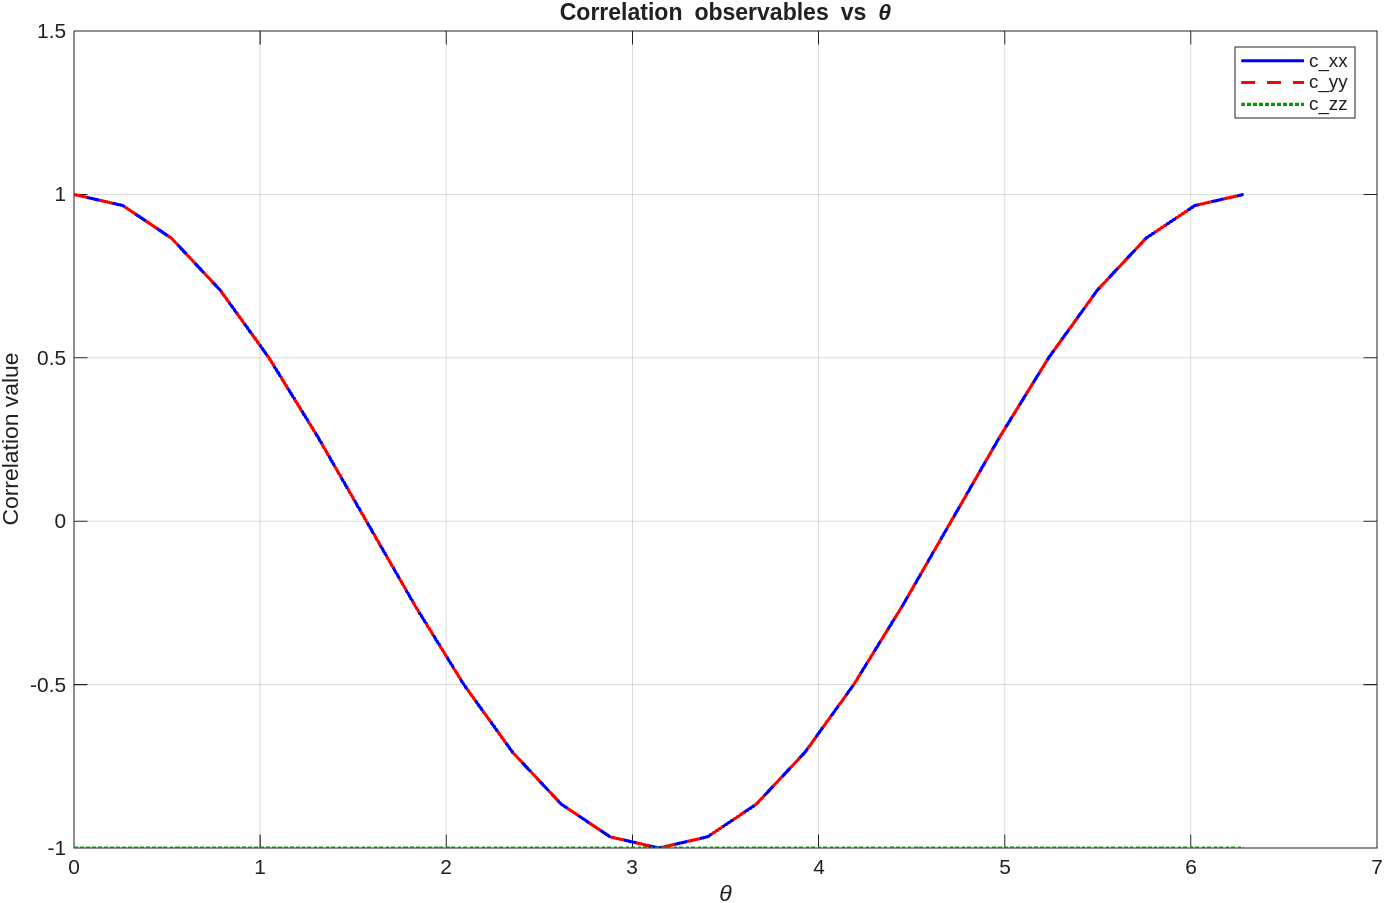
\includegraphics[width=0.75\linewidth]
    {../Images/Experiment_1/correlation_observables_theta.png}
    \caption{
    Numerical evaluation of the correlation observables \(c_{xx}\), \(c_{yy}\), and \(c_{zz}\) as functions of the relative phase \(\theta\).
    }
    \label{fig:experiment1_correlations}
\end{figure}

\begin{figure}[h]
    \centering
    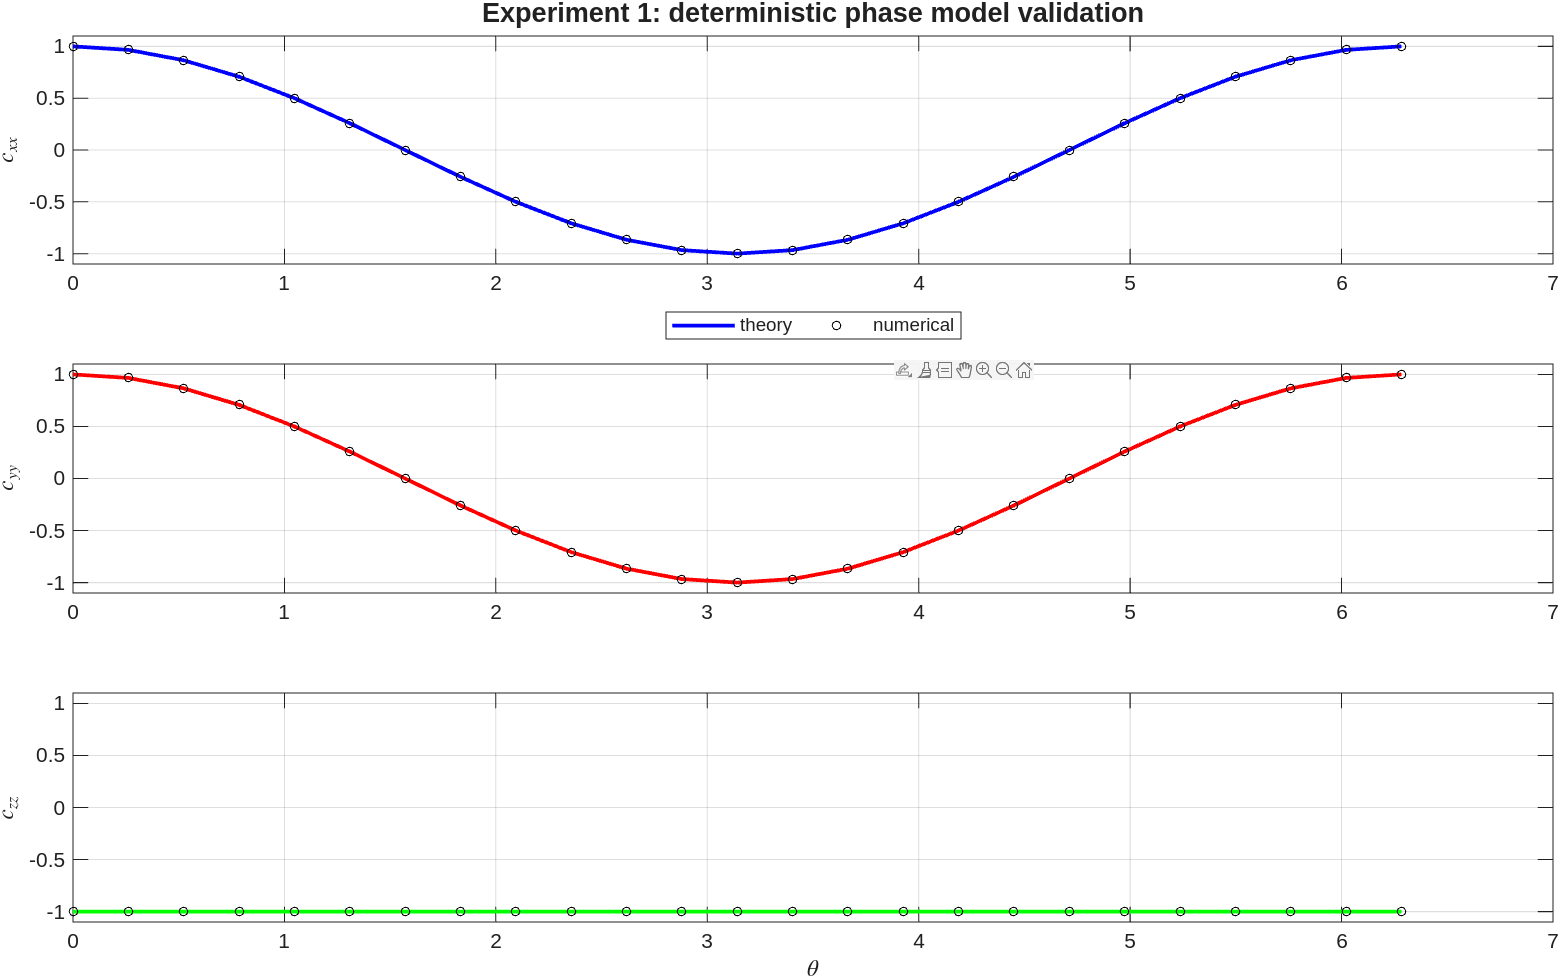
\includegraphics[width=0.75\linewidth]{../Images/Experiment_1/experiment_1_theory_vs_experiment.png}
    \caption{
    Comparison between numerical simulation and analytical predictions for the correlation observables \(c_{xx}\), \(c_{yy}\), and \(c_{zz}\) as functions of \(\theta\).
    The analytical model predicts \(c_{xx} = c_{yy} = \cos\theta\) and \(c_{zz} = -1\), in full agreement with the numerical results.
    }
    \label{fig:experiment1_validation}
\end{figure}

\subsubsection{Discussion}

The numerical results are in full agreement with the analytical predictions. In particular,
\begin{itemize}
    \item \(c_{xx}\) and \(c_{yy}\) exhibit the expected cosine dependence on \(\theta\),
    \item \(c_{zz}\) remains fixed at \(-1\) over the entire sweep.
\end{itemize}

This confirms that, within the reduced model, the fiber acts as an effective relative phase shifter. The state remains pure and maximally entangled for every fixed value of \(\theta\), while its measurable two-photon correlations vary continuously with the phase.

%--------------------------------------------------------

\subsection{Experiment 2: Random Phase Ensemble}

\subsubsection{Objective}

The second experiment extends the deterministic phase model by introducing random phase realizations \(\theta_k\), motivated by the fact that in realistic fibers birefringence fluctuations can produce stochastic phase shifts.

Instead of a single pure state, the system is described by an ensemble of phase-dependent states
\[
\{ |\psi(\theta_k)\rangle \}_{k=1}^{N}.
\]

The objective is to determine how ensemble averaging modifies the observable correlation structure.

\subsubsection{Ensemble Model}

Each realization is given by
\[
|\psi(\theta_k)\rangle
=
\frac{1}{\sqrt{2}}
\left(
|01\rangle + e^{i\theta_k}|10\rangle
\right),
\]
and the ensemble density matrix is defined as
\[
\rho_{\mathrm{ensemble}}
=
\frac{1}{N}
\sum_{k=1}^{N}
|\psi(\theta_k)\rangle\langle \psi(\theta_k)|.
\]

This construction represents the effective state obtained when the phase fluctuates across realizations and the measurement probes only the statistical average.

\subsubsection{Analytical Predictions}

The ensemble-averaged correlation observables satisfy
\[
c_{xx} = \langle \cos\theta \rangle,\qquad
c_{yy} = \langle \cos\theta \rangle,\qquad
c_{zz} = -1,
\]
where the average is taken over the adopted phase distribution.

Thus, the longitudinal correlation remains unchanged, while the transverse correlations are reduced according to the statistical phase coherence retained by the ensemble.

\subsubsection{Numerical Results}

Three representative phase distributions are considered:
\begin{itemize}
    \item constant phase,
    \item uniform distribution,
    \item Gaussian distribution.
\end{itemize}

\begin{figure}[h]
    \centering
    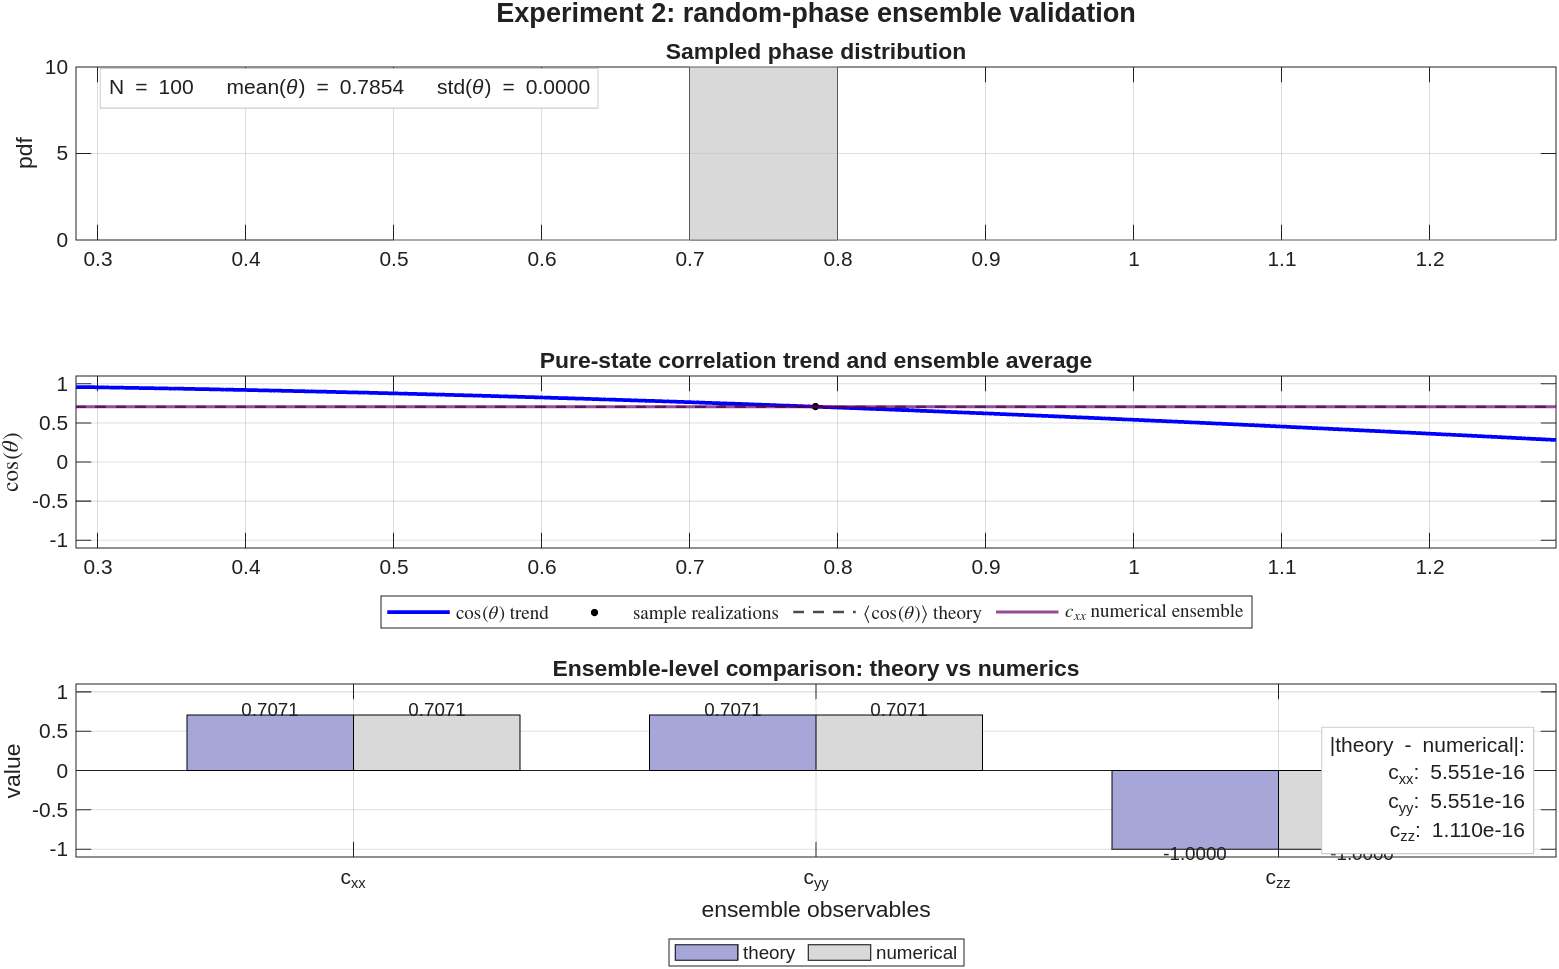
\includegraphics[width=0.9\linewidth]{../Images/Experiment_2/experiment_2_constant_distribution.png}
    \caption{
    Experiment 2 results for a constant phase distribution.
    In this case, the ensemble reduces to a single deterministic phase realization.
    }
    \label{fig:experiment2_constant}
\end{figure}

\begin{figure}[h]
    \centering
    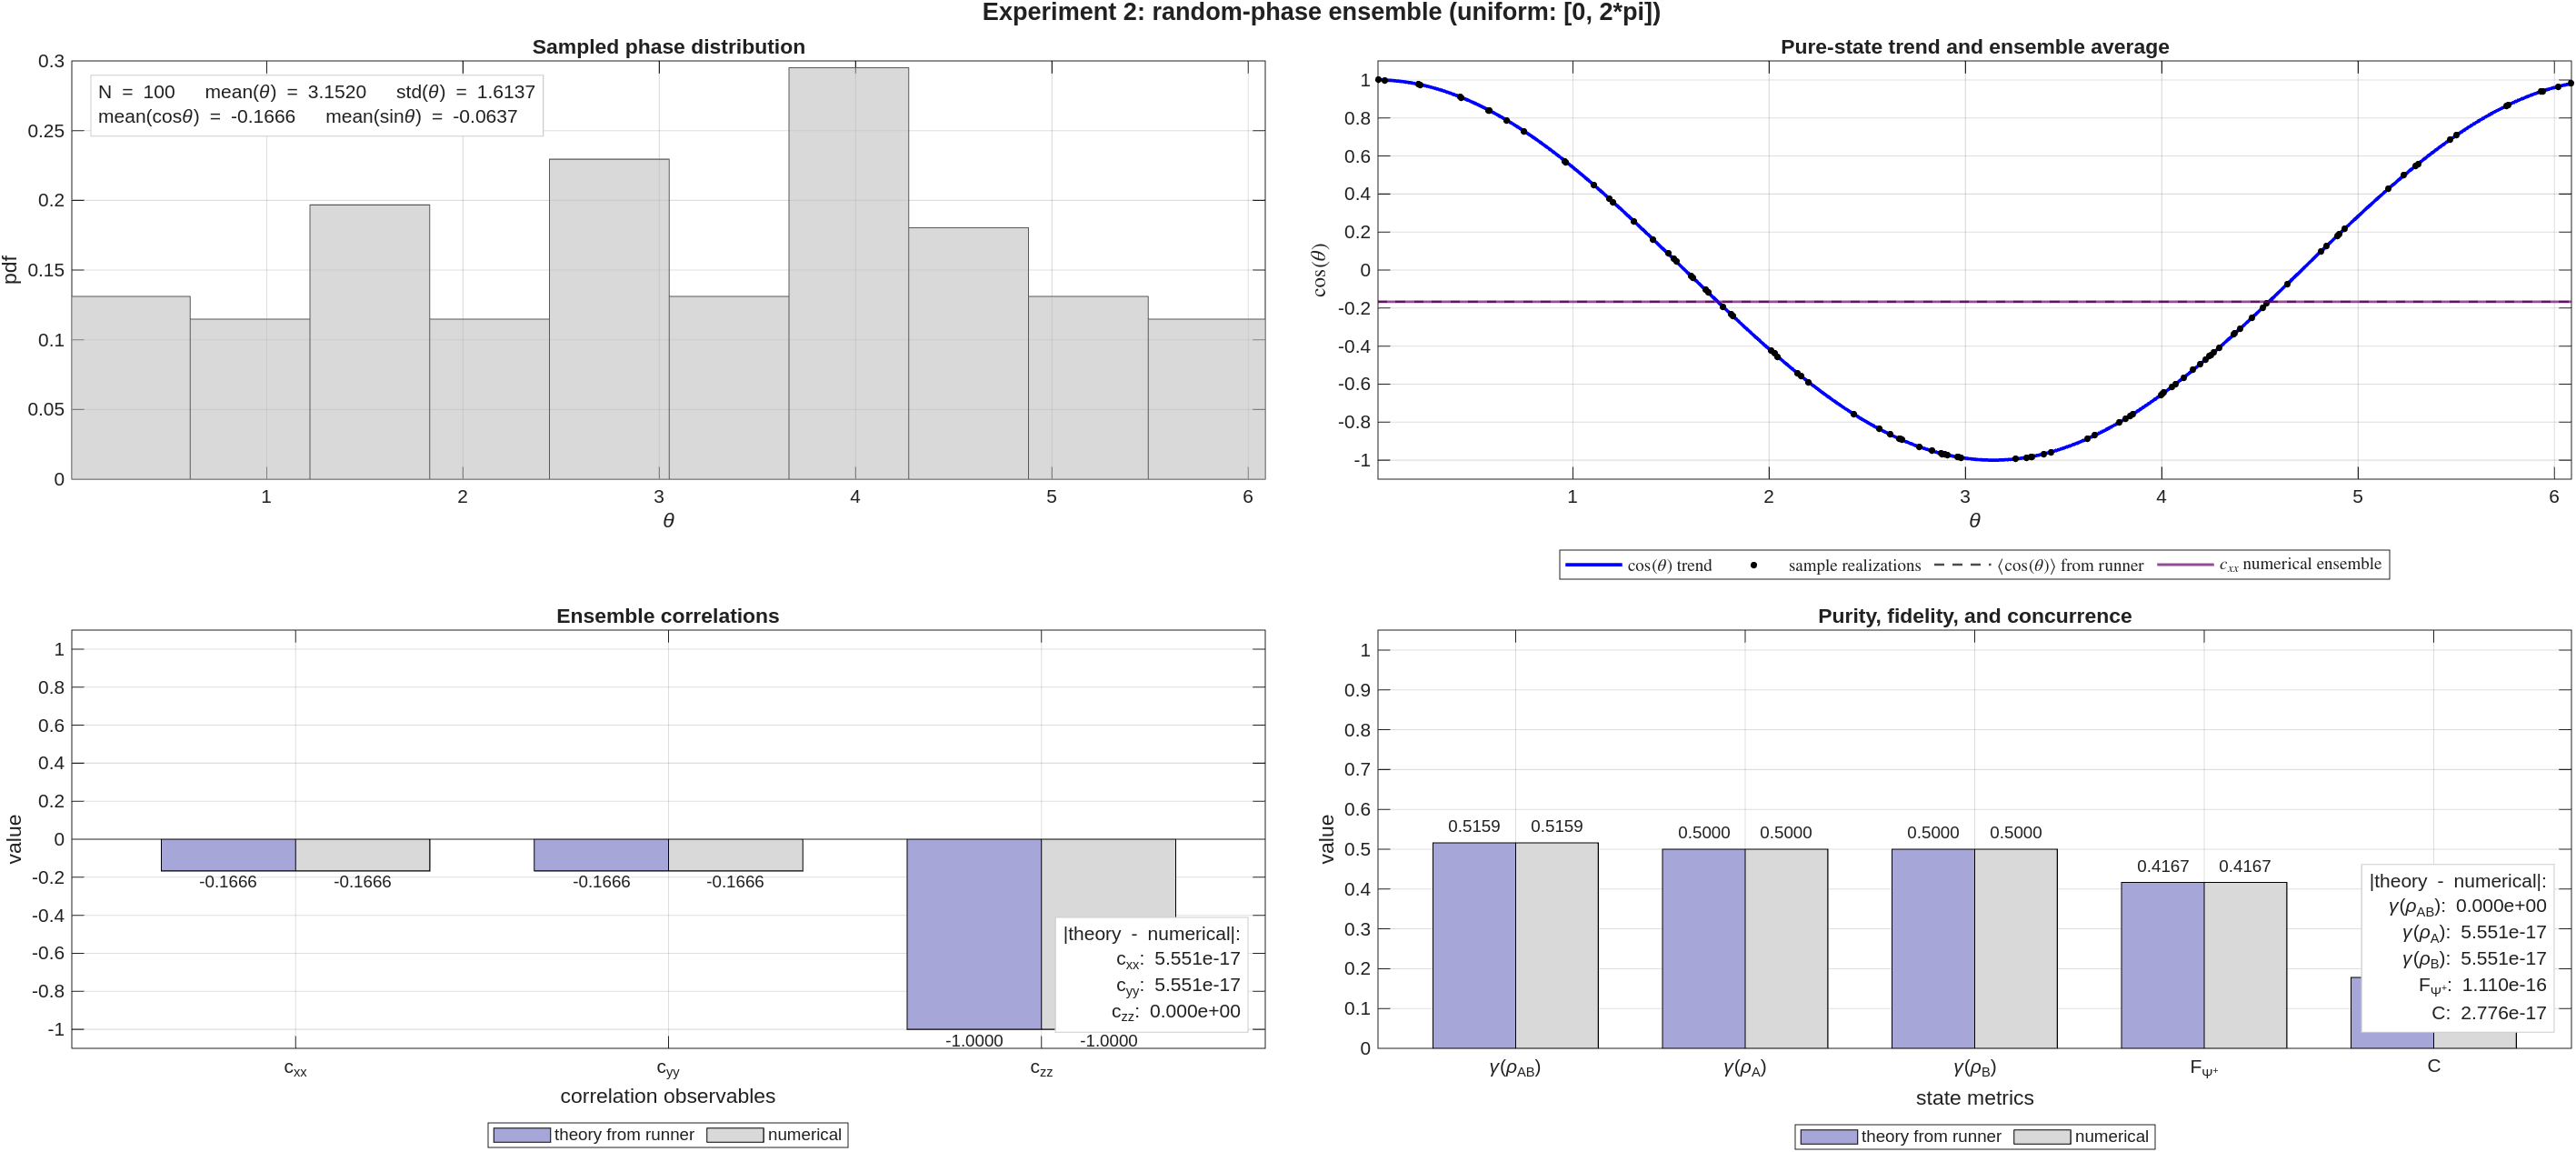
\includegraphics[width=0.9\linewidth]{../Images/Experiment_2/experiment_2_uniform_distribution.png}
    \caption{
    Experiment 2 results for a uniform phase distribution.
    The transverse correlations are reduced by phase averaging, while \(c_{zz}\) remains fixed.
    }
    \label{fig:experiment2_uniform}
\end{figure}

\begin{figure}[h]
    \centering
    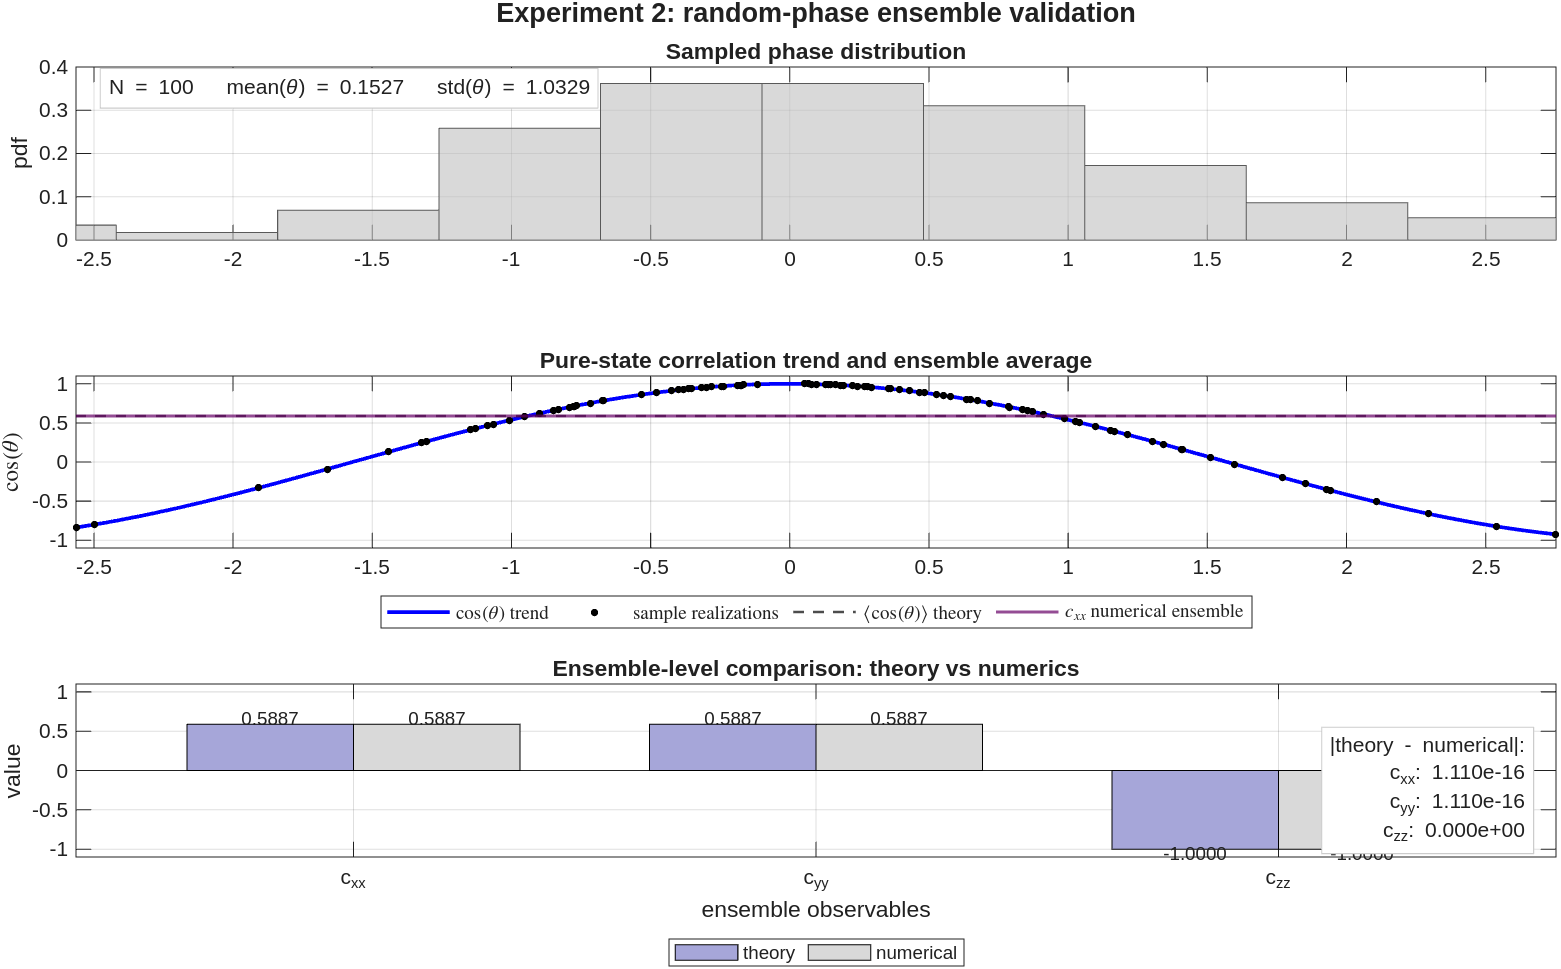
\includegraphics[width=0.9\linewidth]{../Images/Experiment_2/experiment_2_normal_distribution.png}
    \caption{
    Experiment 2 results for a Gaussian phase distribution.
    The amount of residual transverse correlation depends on the concentration of the sampled phases.
    }
    \label{fig:experiment2_gaussian}
\end{figure}

\subsubsection{Discussion}

The numerical results show a clear transition from coherent deterministic behavior to ensemble-averaged mixed-state behavior:
\begin{itemize}
    \item for constant \(\theta\), the model reproduces the deterministic behavior of Experiment 1,
    \item for distributed \(\theta\), the magnitudes of \(c_{xx}\) and \(c_{yy}\) are reduced,
    \item for sufficiently broad phase distributions, \(\langle \cos\theta \rangle \to 0\), leading to vanishing transverse correlations.
\end{itemize}

This behavior reflects a loss of observable phase coherence caused by statistical averaging over different phase realizations.

\subsubsection{Physical Interpretation}

Each individual realization \( |\psi(\theta_k)\rangle \) remains a pure maximally entangled state. However, the ensemble average produces a mixed state described by \(\rho_{\mathrm{ensemble}}\). The reduction of transverse correlations is therefore not due to the loss of entanglement within a single realization, but to the averaging process itself.

This corresponds to a physical regime in which the relative phase fluctuates on timescales or across realizations that are not resolved by the measurement process. The experiment therefore provides the first operational transition from a pure-state description to an effective mixed-state description within the simulator.

It is important to distinguish between the loss of observable correlations and the loss of entanglement. While phase averaging reduces the magnitude of measurable correlations, the resulting mixed state may still retain non-classical correlations depending on the underlying distribution.

A full characterization of entanglement in this regime requires the evaluation of appropriate measures such as concurrence or Bell-inequality violations, which are not included in the present stage but can be incorporated in future extensions of the simulator.

%========================================================
\section{References}

\begin{itemize}
    \item M. A. Nielsen and I. L. Chuang, \textit{Quantum Computation and Quantum Information}, Cambridge University Press.
\end{itemize}

\end{document}